\chapter{Konzeption und Implementation}
\section{Anforderungen}
Ziel dieser Arbeit ist es, den Xilinx Microblaze in die bestehende SpartanMC Entwicklungsumgebung zu integrieren. Um dies zu erreichen, muss zunächst der Microblaze in JConfig eingebunden werden. Der CoreGenerator von Xilinx bietet keine Alternative, da lediglich das Microblaze Micro Controller System (MCS) \cite{MCS} zur Verfügung steht. Dies ist ein System bestehend aus einem Microblaze, Speicher und grundlegenden Peripherien, wie einem UART-Core und Timern. Die Konfigurierbarkeit des Microblaze innerhalb des MCS ist stark eingeschränkt. Features wie Caches oder FSL-Interface stehen nicht zur Verfügung und die Pipeline ist immer dreistufig. Da auf die umfangreiche Konfigurierbarkeit und das FSL-Interface nicht verzichtet werden soll, muss der Microblaze in JConfig integriert werden. Um dies zu erreichen, müssen zunächst sowohl eine Hardwarebeschreibung, als auch eine XML-Modulbeschreibung für den Microblaze erstellt werden. Dies ist ebenso erforderlich für den UART IP-Core und den FSL-Bus IP-Core. Bei der Erstellung der Hardware- und der XML-Modulbeschreibung, ist darauf zu achten, dass dem Nutzer es ermöglicht wird, die Parameter der neuen Komponenten konfigurieren zu können.\\
Es ist außerdem erforderlich, dass Anpassungen an der SpartanMC Toolchain vorgenommen werden. Dies ist notwendig, um die automatische Speicherinitialisierung für den Microblaze zu ermöglichen, da die bestehende Methode der Speicherinitialisierung für den SpartanMC nicht ohne Änderungen für den Microblaze anwendbar ist. Desweiteren muss der Compiler für den Microblaze in die Toolchain integriert werden, da einige der Hardwarebeschleuniger über spezielle Instruktionen angesprochen werden. Eine Vielzahl von IP-Cores von Xilinx sind in VHDL verfasst. Da in der SpartanMC Entwicklungsumgebung IP-Cores zum Großteil in Verilog verfasst wurden, ist es gegebenfalls notwendig, Anpassungen an der Toolchain vorzunehmen, um VHDL Designs zu unterstützen.\\
Optional wäre es wünschenswert, die erfolgreiche Paralellisierung eines Microblaze Programms durch \textmu\/Streams zu zeigen. Hierzu wäre es notwendig, 
\textmu\/Streams soweit anzupassen, dass eine entsprechende Hardwarekonfiguration mit den neu integrierten Komponenten erstellt werden kann und
die Aufrufe der Core-Konnektoren durch Aufrufe der FSL-Blöcke ersetzt werden.
\section{Integration in JConfig}
\subsection{Hardware}
Bevor über die Integration nachgedacht werden kann, muss zunächst festgelegt werden, welche Hardware verwendet wird. Über die Jahre hat Xilinx diverse Versionen des Microblaze veröffentlicht. Die Implementationen des Prozessors sind allesamt verschlüsselt und können nur mit entsprechendem Key entschlüsselt werden. Mit der Einführung von Vivado und der Einstellung der Entwicklung von ISE, änderte sich auch die Art der Verschlüsselung, sodass neuere Versionen des Microblaze nicht mehr von der alten Toolchain entschlüsselt werden können. Da die JConfig Toolchain allerdings Gebrauch von der ISE Toolchain macht, kommen für diese Arbeit nur der Microblaze v8.50c oder ältere Versionen in Frage.\\
Ausgehend vom ISE Installationsverzeichnis, ist das Verzeichnis für die IP-Cores an folgender Stelle zu finden: \textit{"14.7/ISE\_DS/EDK/hw/XilinxProcessorIPLib/pcores/"}. Dort sind alle Versionen des Microblaze, sowie alle Versionen der restlichen Hardware abgelegt. Für sämtliche verwendete IP-Cores werden die aktuellsten Versionen verwendet.
\subsection{Hardwarebeschreibung}
\subsubsection{Erzeugung der Hardwarebeschreibung mit XPS}
Um den Microblaze in JConfig integrieren zu können, ist es zunächst notwendig, eine Hardwarebeschreibung zu erstellen, die den Microblaze instanziiert und parametrisiert.
Diese kann entweder manuell erstellt werden oder mit XPS. In XPS kann dazu mit dem Base-System-Builder ein einfaches System erzeugt werden. Ein Beispiel für ein System ohne Peripherie ist in Abbildung \ref{fig:XPS_EXAMPLE} zu sehen.
\begin{figure}[ht!]
\centering
\includegraphics[width=1\linewidth]{./bilder/XPS_EXAMPLE}
\caption{Einfaches mit XPS generiertes System ohne Peripherie}
\label{fig:XPS_EXAMPLE}
\end{figure}
Das System besteht aus einem Micorblaze, zwei LMB, zwei Speichercontrollern (je einen für Daten und einen für Instruktionen), einem Block RAM als Programm- und Datenspeicher, einem AXI4-Light-Bus zur Anbindung von Peripherie, einem Reset-Core, einem Taktgenerator und einem Debug Modul. Um die Komplexität des Systems und somit zusätzliche Fehlerquellen zu reduzieren, werden der AXI4-Light-Bus, der Taktgenerator und das Debug Modul zunächst entfernt. Der AXI4-Bus wird nicht benötigt, da es zunächst in der SpartanMC Entwicklungsumgebung mit dem UART IP-Core nur eine Peripherie geben wird und diese direkt mit dem Prozessor verbunden werden kann. Der Taktgenerator wird nicht benötigt, da JConfig bereits über eigene Taktgeneratoren verfügt und das Debug Modul wird nicht benötigt, um die grundsätzliche Lauffähigkeit eines Microblaze Systems zu gewährleisten, sondern nur um Softwareanwendungen zu debuggen.\\
Nun kann in XPS eine Netzliste erzeugt werden. Als Nebenprodukt werden Wrapperdateien erstellt, die die einzelnen Komponenten mit den, im XPS angegebenen Einstellungen instanziieren. Die erzeugten Dateien werden nach Möglichkeit in der präferierten Sprache erzeugt, allerdings funktioniert dies bei manchen Wrapper Dateien nicht und sie werden in VHDL generiert. Die Top-Level-Beschreibung, welche sämtliche Komponenten instanziiert und miteinander verbindet, kann allerdings auch in Verilog erzeugt werden. Desweiteren besitzt die Top-Level-Beschreibung lediglich die, im XPS als extern makierten Signale als Eingänge und Ausgänge. Die Wrapper Datei für das Block RAM stellt eine Besonderheit dar. Für das Block RAM wird nämlich, entsprechend der angegebenen Größe des Speichers, ein elaboriertes Modell erzeugt. Dieses Modell funktioniert nur für die angegebene Speichergröße und lässt sich ohne großen Aufwand auch nicht ändern. Als Lösung des Problems wird ein generisches Speichermodul in Verilog geschrieben, welches das Verhalten der elaborierten Blöcke nachahmt (siehe \ref{subsubsec:genMem}).\\
Um nun eine konfigurierbare Hardwarebeschreibung zu erhalten, ist es notwendig, den Wrapperdateien und der Top-Level-Beschreibung Parameter hinzuzufügen. So können bei der Instanziierung des Top-Level-Moduls Parameter übergeben werden, die dann wiederum bei der Instanziierung der einzelnen Komponenten des Systems an diese weitergegeben werden können. Ebenso ist es erforderlich, dass Signale die verwendet werden sollen, als Eingänge bzw. Ausgänge der Top-Level-Beschreibung hinzugefügt und über Signale mit der entsprechenden Komponente verbunden werden. Für den Microblaze sind dies zu Beginn, neben Takt- und Reset-Signalen, Signale für den Programm- und Datenspeicher, AXI4-Signale und Signale, die dem FSL-Interface zuzuschreiben sind.\\
Unter Berücksichtigung der XML-Modulbeschreibung, ist es notwendig, den Speicher als externes Modul zu handhaben, da die XML-Syntax für Prozessoren keine integrierten Speicher unterstützt. Hierzu werden die Speichercontroller und das Block RAM in einem weiteren Modul zusammengefasst (siehe \ref{subsubsec:genMem}), sodass das Modul für den Microblaze noch aus den Instanzen für den Microblaze selbst, den beiden LMB und dem Reset-Core besteht. Die LMB-Cores erlauben es mehr als einen Speicher an den Microblaze anzuschließen.\\
Welche Parameter für die Konfiguration des Microblaze wichtig sind, wird im nächsten Abschnitt behandelt. 
\subsubsection{Handhabung der Parameter}
In diesem Kapitel wird behandelt, welche Parameter für die Konfiguration des Microblaze-Systems wichtig sind.
Für die Parameter des Microblaze wurde die Tabelle aus dem Abschnitt \textit{MicroBlaze Core Configurability} in Kapitel 3 des Microblaze Datenblattes \cite{MBREF} herangezogen. Parameter, die in der Tabelle nur einen Wert in der Spalte \textit{Allowable Values} haben, werden fest auf diesen Wert gesetzt und können nicht vom Anwender verändert werden. In der Tabelle \ref{tab:MicParam} werden lediglich die Parameter behandelt, welche mehr als einen erlaubten Wert haben, allerdings trotzdem auf einen festen Wert gesetzt werden. Alle anderen Parameter, die nicht genannt werden, stehen dem Nutzer zur freien Konfiguration zur Verfügung. Erklärungen zu den Bedeutungen der einzelnen Parametern werden in Kurzform in der XML-Modulbeschreibung hinterlegt, sodass der Nutzer während der Erstellung eines Systems weiß, welche Funktion die einzelnen Parameter haben. Für detailliert Beschreibungen sei noch einmal auf das Datenblatt des Microblaze verwiesen \cite{MBREF}.
\begin{table}[ht!]
	\begin{tabular}{|l|c|p{10cm}|}
		\hline \textbf{Parameter} & \textbf{Wert} & \textbf{Beschreibung} \\ 
		\hline C\_LOCKSTEP\_SLAVE & 0 & Im Lockstep Modus können zwei oder mehrere \newline Microblaze das selbe Programm ausführen und die Ergebnisse miteinander vergleichen, um Hardwarefehler zu erkennen. Wird nicht benötigt.\\ 
		\hline C\_ENDIANNESS & 1 & Endianness wird auf Little Endian festgelegt. In XPS lässt sich dieser Wert nicht manuell verändern, dementsprechend wird auch unter JConfig darauf verzichtet.\\ 
		\hline C\_D\_AXI & 1 & Das AXI-Daten-Interface kann verwendet werden. \\ 
		\hline C\_I\_AXI & 1 & Das AXI-Instruktionen-Interface kann verwendet werden. (Nützlich bei externen Speicher) \\ 
		\hline C\_D\_PLB & 0 & Da bereits AXI verwendet wird, wird der PLB Bus nicht gebraucht und deshalb deaktiviert. \\ 
		\hline C\_I\_PLB & 0 & Siehe vorheriger Eintrag. \\ 
		\hline C\_D\_LMB & 1 & Das LMB-Daten-Interface kann verwendet werden. \\ 
		\hline C\_I\_LMB & 1 & Das LMB-Instruktionen-Interface kann verwendet werden. \\ 
		\hline C\_IPLB\_BUS\_EXCEPTION & 0 & Da der PLB nicht verwendet wird, werden die Exceptions auch nicht benötigt. \\ 
		\hline C\_DPLB\_BUS\_EXCEPTION & 0 & Siehe vorheriger Eintrag. \\ 
		\hline C\_ADDR\_TAG\_BITS & 17 & Das Datenblatt gibt kaum nützliche Informationen zu diesem Parameter, daher wird er auf den Default-Wert festgesetzt. \\ 
		\hline C\_DCACHE\_ADDR\_TAG & 17 & Siehe vorheriger Eintrag. \\ 
		\hline C\_USE\_EXT\_BRK & 0 & Siehe vorheriger Eintrag. \\ 
		\hline C\_USE\_EXT\_NM\_BRK & 0 & Siehe vorheriger Eintrag. \\ 
		\hline 
	\end{tabular}
	\centering
	\caption{Parameter des Microblaze die mehr als einen erlaubten Wert haben, aber dennoch auf einen Wert festegelegt werden.}
	\label{tab:MicParam}
\end{table}
Neben dem Microblaze werden mit einem generischen Speichermodul, einem UART-Modul und einem FSL-Modul noch drei weitere Hardwarekomponenten für JConfig erstellt, die parametrisiert werden können. Welche Parameter zur Verfügung stehen und was diese bewirken, ist in den Tabellen \ref{tab:MemParam}, \ref{tab:UARTParam} und \ref{tab:FSLParam} aufgeführt.

\begin{table}[ht!]
	\begin{tabular}{|l|p{10cm}|}
		\hline \textbf{Parameter} & \textbf{Beschreibung} \\ 
		\hline C\_FAMILY & Dieser Parameter wird von Xilinx IP-Cores verwendet, um, je nach verwendeter Hardware, vorhandene Primitives zu instanziieren. \\ 
		\hline RAMBLOCKS & Ähnlich wie für den Speicher des SpartanMC, kann angegeben werden, wie viel RAM instanziiert werden soll. Ein Block ist jeweils 2KB groß. Es können nur Größen gewählt werden, die einer Potenz von Zwei entsprechen, da mit jeder Vergrößerung des Speichers sich die Anzahl der Bitlanes verdoppelt.\\ 
		\hline C\_BASEADDRESS & Gibt die Startaddresse des Speichers an.\\ 
		\hline 
	\end{tabular}
	\centering
	\caption{Parameter des Speichermoduls für den Microblaze.}
	\label{tab:MemParam}
\end{table}

\begin{table}[ht!]
	\begin{tabular}{|l|p{10cm}|}
		\hline \textbf{Parameter} & \textbf{Beschreibung} \\ 
		\hline C\_S\_AXI\_ACLK\_FREQ\_HZ & Frequenz des Taktsignals, welches automatisch aus dem Takt abgeleitet wird.\\ 
		\hline C\_FAMILY & Dieser Parameter wird von Xilinx IP-Cores verwendet, um, je nach verwendeter Hardware, vorhandene Primitives zu instanziieren.\\ 
		\hline C\_BAUDRATE & Für die Übertragung verwendete Baudrate. Eine Auswahl von Werten zwischen 110 und 921600 steht zur Verfügung. \\ 
		\hline C\_DATABITS & Anzahl der zu übertragenden Bits pro Frame. Werte von 5 bis 8 sind möglich. \\ 
		\hline C\_USE\_PARITY & Gibt an, ob ein Paritätsbit mit übertragen wird. \\ 
		\hline C\_ODD\_PARITY & Gibt an, ob die Parität gerade oder ungerade ist. \\ 
		\hline 
	\end{tabular}
	\centering
	\caption{Parameter des UART-Cores.}
	\label{tab:UARTParam}
\end{table}

\begin{table}[ht!]
	\begin{tabular}{|l|p{10cm}|}
		\hline \textbf{Parameter} & \textbf{Beschreibung} \\ 
		\hline C\_EXT\_RESET\_HIGH & Gibt an, ob das externe Reset-Signal high-aktiv oder low-aktiv ist.\\ 
		\hline C\_ASYNC\_CLKS & Gibt an, ob das FSL-Interface synchron oder asyncron betrieben werden soll.\\ 
		\hline C\_IMPL\_STYLE & Wenn dieser Parameter auf 0 gesetzt ist, wird der FIFO-Speicher mit LUT RAMs implementiert, andernfalls mit Block RAMs.   \\ 
		\hline C\_USE\_CONTROLL & Bestimmt, ob das Steuerbit mit übertragen wird oder nicht.\\ 
		\hline C\_FSL\_DWIDTH & Ist auf 32 Bit festgelegt, da andere Datenbreiten im Zusammenhang mit dem Microblaze wenig sinnvoll sind. \\ 
		\hline C\_FSL\_DEPTH & Beschreibt die Größe des FIFO-Speichers. Diese ist von den Parametern C\_ASYNC\_CLKS und C\_IMPL\_STYLE abhängig. C\_ASYNC\_CLKS=0 => 1-8192. C\_ASNYNC\_CLKS=1 und C\_IMPL\_STYLE=0 => 16-128. C\_ASNYNC\_CLKS=1 und C\_IMPL\_STYLE=1 => 512-8192. Ist C\_ASNYNC\_CLKS=1 muss die Größe außerdem einer Potenz von Zwei entsprechen.\\ 
		\hline C\_READ\_CLOCK\_PERIOD & Wird automatisch aus dem Taktsignal berechnet. Wird genutzt um Timing Constraints für den asynchronen Pfad durch LUT RAMs zu erzuegen \\
		\hline 
	\end{tabular}
	\centering
	\caption{Parameter des FSL-Cores.}
	\label{tab:FSLParam}
\end{table}

\subsubsection{Implementation eines generischen Speichermoduls} \label{subsubsec:genMem}
Bevor über eine Implementation eines generischen Speichermoduls nachgedacht werden kann, sollte zunächst die Struktur, des von Xilinx verwendeten Speichers erläutert werden. Hierzu wird Abbildung \ref{fig:XilinxMEM} herangezogen.
\begin{figure}[ht!]
\centering
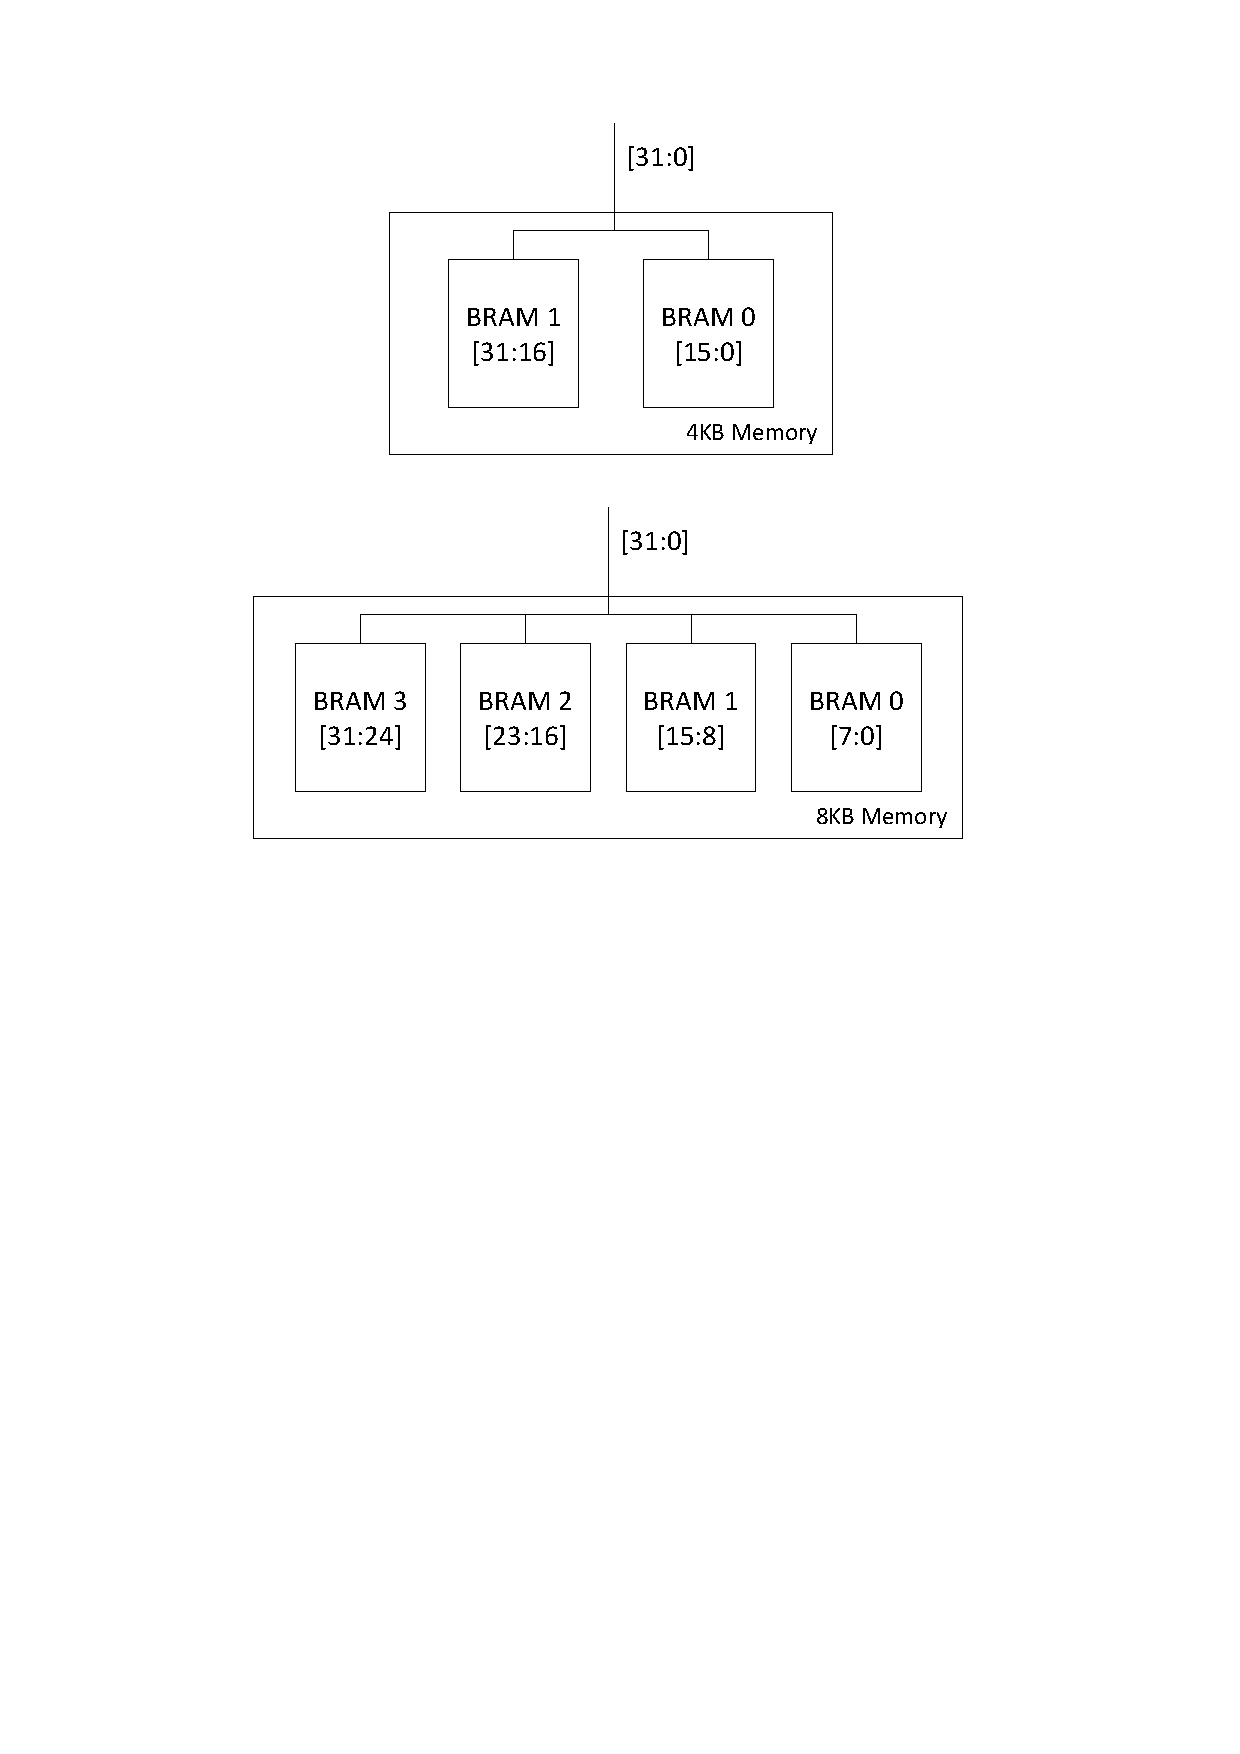
\includegraphics[width=0.7\linewidth]{./bilder/XilinxMEM}
\caption{Speicherstruktur der von Xilinx generierten Speichermodule}
\label{fig:XilinxMEM}
\end{figure}
In der Abbildung sind einfache Blockschaltbilder für einen 4KByte und einen 8KByte großen Speicher dargestellt. Angefangen bei einer Mindestgröße von 2KByte verdoppelt sich die Anzahl der Block RAMs bei jeder Vergrößerung. Dabei halbiert sich jeweils die Größe der Bitlanes bis hin zu einem Minimum von eins bei einer maximalen Speichergröße von 64KByte. Die vom XPS generierten Modelle instanziieren immer eine fixe Anzahl an Block RAMs, sodass es nicht möglich ist, mit der selben Methode wie beim Microblaze eine generische Parametriserbarkeit herzustellen. Daher muss, auf Grundlage der elaborierten Modelle, ein generisches Speichermodul geschrieben werden, dessen Größe über einen Parameter festgelegt werden kann.\\
Um dies zu erreichen, wird ein Verilog-Modul geschrieben, welches die Parameter \textit{RAMBLOCKS} und \textit{C\_FAMILY} hat. Über eine for-Schleife in einer generate-Umgebung werden entsprechend des Parameters \textit{RAMBLOCKS} dual-ported Block RAMS instanziiert. Einen Port handhabt Daten und der andere Instruktionen. Eine Funktion berechnet dabei aus dem Parameter die Breite der einzelenen Bitlanes. Um die Signalverbidungen zu realisieren, werden wires und regs deklariert, deren Größe mit \textit{RAMBLOCKS} skaliert. Über Indexing wird innerhalb der for-Schleife die Realisierung der einzelnen Bitlanes vorgenommen. Für das 4-Bit breite Write-Enable-Signal wird zusätzliche Kombinatorik hinzugefügt, da die Handhabung nicht durch einfaches Indexing umgesetzt werden kann.\\
Zuletzt werden der Speicher und zwei Speichercontroller in einer Top-Level-Beschreibung instanziiert und miteinander verbunden.

\subsection{Modulbeschreibungen}
Für den Microblaze, den Speicher, den UART-Core und den FSL-Core müssen nun XML-Modulbeschreibungen erstellt werden. Nachfolgend werden alle hierzu notwendigen Schritte besprochen:
\begin{itemize}
\item \textbf{Microblaze}: Der Microblaze wird in der Beschreibung als Prozessor kategorisiert. Neben den Wrapperdateien für den Microblaze, den LMBs und dem Reset-Modul müssen noch Pfadangaben für die HDL-Dateien der Implementationen dieser Cores angegeben werden. Um dies umzusetzen, wurde die XML-Syntax mit \textit{externalRoot} um ein neues Konstrukt erweitert. Dieses Konstrukt erlaubt es absolute Pfade außerhalb des Default-Verzeichnisses anzugeben und wurde nicht im Rahmen dieser Arbeit ergänzt, sondern von einem Kommilitonen, der zum Zeitpunkt dieser Arbeit für die Wartung von JConfig verantwortlich war. Alle Dateien, die sich im Scope eines \textit{externalRoot}-Konstruktes befinden, verwenden den angegeben Pfad als Ausgangsverzeichnis. Im Rahmen dieser Arbeit, wurde in der Klasse \textit{HDLDescription} im Package \textit{de.tu\_darmstadt.rs.spartanmc.devxml.descriptions.generic} eine Anpassung vorgenommen, die Umgebungsvariablen in Pfadangaben auflöst. So wird über die Umgebungsvariable \textit{XILINX\_ROOT} plattformunabhängig der Pfad zu den HDL-Dateien angegeben. Desweiteren ist es möglich, einen Namen für eine VHDL-Library anzugeben, unter dem die entsprechenden Dateien zusammengefasst werden. Dies ist für die Xilinx Cores notwendig, da innerhalb der Implementationen einige Libraries referenziert werden. Außerdem verkürzen Libraries die Kompilierzeit während der Simulation.\\
Es folgen daraufhin die Angaben der Parameter. Hierbei wurde darauf geachtet, dass die Gruppierung der Parameter in ähnlicher Weise erfolgt, wie es im Wizard des XPS der Fall ist. Die Parameter werden desweiteren mit einem Beschreibungstext versehen, sodass sich die Funktion für den Anwender bei der Parametrisierung erschließt. Außerdem haben die Konfigurationsmöglichkeiten einiger Parameter eine relativ geringe Aussagekraft. So lässt sich beispielsweise der Modus der MMU über einen Parameter steuern, der die Werte null bis drei annehmen kann. Um mehr Informationsgehalt zu vermitteln, wurde ein String-Parameter eingeführt, der die Werte \textit{``None''}, \textit{``Usermode''}, \textit{``Protection''} und \textit{``Virtual''} annehmen kann. Innerhalb der Top-Level-Verilog-Beschreibung wird dann über eine Aliasing-Funktion der String zu einem Integer umgewandelt. Dies wird für weitere Parameter durchgeführt, bei denen die Aussagekraft der Auswahlmöglichkeiten zu wenig Information vermittelt.\\
Desweiteren schließen sich einige Konfigurationsmöglichkeiten gegenseitig aus. So ist es beispielsweise nicht möglich, die MMU zu verwenden, wenn der Parameter \textit{C\_AREA\_OPTIMIZED} gesetzt ist. Um eine Auswahl in einem solchen Fall zu verhindern, wird das Konstrukt \textit{relevantIf} in Zusammenhang mit einer invertierten Version von \textit{C\_AREA\_OPTIMIZED} verwendet.\\
Darauf folgen Bus-Deklarationen für Speicherbusse und FSL-Busse (siehe \ref{subsec:BusDesc}), wie auch Signal-Deklarationen für Takt, Reset und dem AXI-Bus.\\
Abschließend wird das \textit{addressLayout} für den Daten- und Instruktionsspeicher definiert. Für Peripherie wurde noch kein Adressraum festgelegt, da es bis lang nur den UART-Core als Peripherie gibt, und dieser direkt mit dem Microblaze verbunden wird. Sobald ein AXI-Bus in JConfig verfügbar ist, muss auch ein Adressraum für die Peripherie hinzugefügt werden.
\item \textbf{Speicher}: Die Erstellung der Modulbeschreibung für den Speicher erfolgt ähnlich wie für den Microblaze. Die verfügbaren Parameter sind in Tabelle \ref{tab:MemParam} aufgelistet. Der Speicher wird allerdings als Memory kategorisiert und hat mit dem \textit{memory}-Konstrukt eine Besonderheit. Mit \textit{memory} wird die Größe des Speichers, das Namensschema der Speicherinstanzen und die Reset-Werte beschrieben. Außerdem kann angegeben werden, ob der Speicher eine Aufteilung zwischen Daten und Instruktionen vorsieht. Diese Informationen werden später bei der Erzeugung der Memory-Map benötigt.
\item \textbf{UART}: Auch hier wird die Modulbeschreibung nach ähnlichem Muster erstellt. Der UART-Core ist allerings als Peripherie kategorisiert. Über das \textit{registers}-Konstrukt können Angaben zu Registern innerhalb des Cores gemacht werden, die später während der Erstellung der Software verwendet werden können. Im Rahmen dieser Arbeit konnte dieses Konstrukt für die UART allerdings nicht mehr erstellt werden. Die zur Verfügung stehenden Parameter sind in Tabelle \ref{tab:UARTParam} zu finden.
\item \textbf{FSL}: Der FSL-Core wird als Core Interconnect kategorisiert und hat keine weiteren Besonderheiten. Die Parameter sind in Tabelle \ref{tab:FSLParam} aufgelistet.
\end{itemize}

\subsection{Busbeschreibungen}\label{subsec:BusDesc}
Um das Verbinden einzelner Komponenten zu vereinfachen, werden zusammengehörige Signale zu einem Bus zusammengefasst. Im Folgenden wird auf die, im Rahmen dieser Arbeit erstellten Busbeschreibungen eingegangen:
\begin{itemize}
\item \textbf{FSL-Busse}: Für den FSL-Bus werden zwei neue Busbeschreibungen in Form von XML-Dateien erstellt. Ein Bus beschreibt die Verbindungen für das Master-Interface und der andere die Verbindungen für das Slave-Interface (siehe Abbildung \ref{fig:FSLBSB}). Die Busbeschreibungen enthalten Defintionen für \textit{masterPorts} und \textit{slavePorts}, sowie alle dazugehörigen Signale, deren Richtung und Datenbreite.
Bei der Deklaration innerhalb der Modulbeschreibung für den Microblaze wird darauf geachtet, das die einzelnen Signale in den Busbeschreibungen mit der Option \textit{combineUsing="parallel"} versehen sind. Dies bewirkt, dass die einzelnen Signale, der bis zu 16 FSL-Busse konkateniert und so an den Microblaze weitergeleitet werden.
\item \textbf{Speicherbusse}: Sowohl alle für den Datenport des Speichers relevanten Signale, sowie alle für den Instruktionsport relevanten Signale, werden zu je einem Bus zusammengefasst. Die Beschreibung erfolgt nach ähnlichem Schema wie bei den FSL-Bussen. Die \textit{masterPorts} fassen alle Signale auf Seiten des Microblaze zusammen, während \textit{slavePorts} alle Signale des Speichers umfasst.
\end{itemize}
Für die AXI-Signale wurden im Rahmen dieser Arbeit noch keine Busse erstellt, dies sollte allerdings mit der Integration eines AXI-Bus-IP-Cores nachgeholt werden.

\section{Integration in die SpartanMC Toolchain}
\subsection{Ausgangslage}
Der Microblaze und alle notwendigen Peripherien sind in JConfig eingebunden. Mit den von JConfig generierten Dateien, kann die Toolchain allerdings noch kein funktionsfähiges Bitfile erzeugen, da die Speicherarchitekturen des SpartanMC und des Microblaze verschieden sind. Der Speicher des SpartanMC ist so aufgebaut, dass dem Parameter \textit{RAMBLOCKS} entsprechend Block RAMs instanziiert werden, dessen Bitlanes immer 18-Bit breit sind. So wird bei jedem Speicherzugriff auf genau ein Block RAM zugegriffen und nicht auf alle, wie beim Microblaze.\\
Das Tool Initramj der SpartanMC Entwicklungsumgebung wird zur Speicherintialisierung für den SpartanMC verwendet und ist auf die vorher beschriebene Speicherstruktur angepasst. Das Tool ist unter anderem in der Lage, Speicherinitialisierungen in Form von UCF-Dateien, Verilog-Dateien oder Bitfile-Updates durchzuführen. Hierzu benötigt es eine ELF-Datei und eine Memory-Map in Form einer Datei namens \textit{memory.xml}. Es wäre also denkbar, Initramj dahingehend anzupassen, dass es auch die Speicherinitilaisierung für die 32-Bit-Speicherarchitektur des Microblaze durchführen kann. Dies hätte den Vorteil, dass die Speicherininitialisierung gekapselt von einem einzigen Tool gehandhabt würde und somit kaum Änderungen an den Makefiles notwendig wären.\\
Eine Alternative zu Initramj stellt die Speicherinitialisierung mit dem Xilinx-Tool data2mem dar. Hierfür müsste JConfig allerdings eine weitere Memory-Map in Form einer BMM-Datei erzeugen. Desweiteren müssten die Makefiles angepasst werden, sodass sie data2mem aufrufen. Im Rahmen dieser Arbeit wurde die Variante mit data2mem umgesetzt, da der Aufwand zur Anpassung von Initramj als zu hoch eingeschätzt wurde.\\
Desweiteren ist es notwendig, den Microblaze GCC in die Toolchain zu integrieren, da der SpartanMC Compiler keinen, vom Microblaze ausführbaren Code generieren kann. Um dies zu erreichen, müssen weitere Änderungen an den Makefiles vorgenommen werden.
\subsection{Erzeugung der BMM-Datei}

\subsection{Anpassungen in der Toolchain zur Speicherinitialisierung}

\subsubsection{Speicherinitialisierung mit UCF-Datei}

\subsubsection{Aktualisierung des Bitfiles}

\subsubsection{Speicherintialisierung für die Simulation}

\subsection{Unterstützung von Libraries in der Simulation}

\subsection{Integration des Microblaze GCC}

